\chapter{Experimental System and Setup}
Because of the unresolved issues with stimuli generation the experiment setup has not been
employed on live neural tissue.
As a consequence, the current experimental setup is designed to be easy to
modify whenever testing becomes possible and to verify functionality of the rest
of the system.
Consequentially, the focus on this section is the capabilities for experimentation
provided by the system, and the parameter space that can be explored.\par
%
When leaving out all implementation details the setup for conducting experiments
provided by SHODAN and MEAME shown in \ref{figExperimentLoop} becomes much simpler.
The setup can be divided into three separate components.
The first two components are the \emph{primary} and \emph{secondary} dataloop
which both interact with the third component, the \emph{robot control} module.
The focus of this chapter is the role each of the three components of an
experiment serve, and a survey of the parameter space which can be explored. 
\begin{figure}[h!]
  \centering
  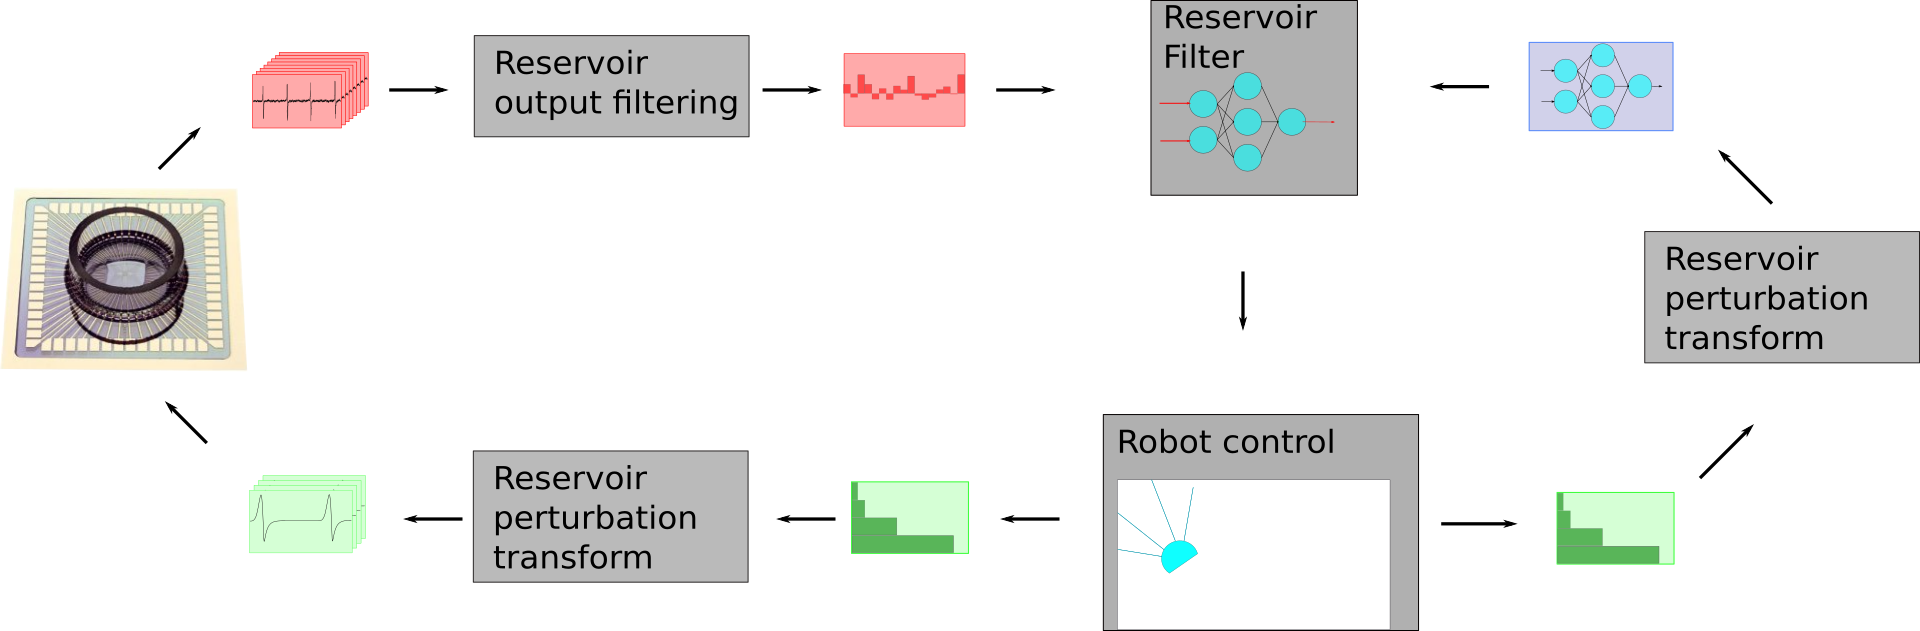
\includegraphics[width=1\textwidth]{fig/experimentLoop.png}
  \caption{Rough sketch.
    Some wavez
  }
  \label{figExperimentLoop}
\end{figure}
%
\subsubsection{Deviation From Classical Reservoir Computing}
Before going further it is necessary to clarify where the experimental setup
deviates from a classical reservoir computer setup, as well as definig the
terminology.
Henceforth, a \emph{run} is defined as continously running the reservoir
computer with no outside intervention for some duration of time.
An \emph{experiment} can consist of several runs in which the dataloop between
reservoir and reservoir computer is restarted between runs. 
Finally, the goal of an experiment is to optimize the performance at a given
\emph{task} according to some criteria.
%% Skrive noe mer autistisk om perf measurement?
In the classic RC setup the input layer is not altered during an individual run,
instead it is modified between runs, and the resulting experiment iterates
towards an input filter capable of solving some task specified by the
experiment.
From this angle the classic model is very close to the one shown in
\ref{figExperimentLoop}, but there is one major difference, namely that the two
loops run in a \emph{sequential} lockstep fashion 
rather than in \emph{parallel}, or \emph{on-line} as is the case with the cyborg.
Running each loop sequentially makes more sense than parallel when the reservoir
can be reset to an initial state, but this is not 
the case with live tissue whose topology and function evolves both over time,
and as a response to previous experiments. This effect is exacerbated by the
imperfect measurement of electrodes, where a cluster of neurons can seemingly
vanish by physically moving away from an electrode.
\subsubsection{A Sample Experiment}
Before detailing the component systems it is useful to describe an experiment to
make the intended operation of the system clearer when described in detail in
the following sections.\par
Before starting parameters that are considered static are pulled from a
configuration file and a database record with the current configuration is
created.
These parameters describe constants such as max electrode stimuli frequency,
agent turn rate and similar, and once good values have been found they should
not be altered (which is why they are stored in a file).
When the experiment is started the secondary dataloop will ``cold start'' the
system by generating a set of random #input layers. The main dataloop will then start
pulling data from the reservoir and feed it into the generated input layer,
which in turn controls the robot.
Output from the robot is then simultaneously sent through both dataloops, the
primary loop uses it to generate reservoir perturbations while the secondary
loop uses it to evaluate the current input layer.
After all the randomly generated generated networks have been evaluated the
secondary dataloop creates a new set of input layers based on the most
successful layers from the previous generation.
This keeps repeating until the experiment is terminated, hopefully after
converging on a set of input layers capable of adequately solving the presented
task.
Since the system stores all data in a database it is possible to play back
previous recordings without the system being aware of this (of course the
perturbation will not do anything in this case), but it helps debugging and
ensures that all relevant information is stored in the database.
For convenience all the configuration can be done through a web interface which
supports loading previously stored settings, visualizing live data and give
diagnostics in case of equipment failure. 
% TODO figur av webshit
\section{Primary Data Loop}
A more detailed view of the data loop is shown in figure \ref{figDataLoop}.
Since the primary dataloop interacts with the robot control it must be part of
the diagram, but it is considered a separate component for configuration
purposes.
The two configurable parts of the primary dataloop is shown in the figure as the
reservoir output filter and the perturbation transform.
In the classical RC model the #input layer is typically illustrated a single
transform, however when 
dealing with a physical reservoir it is useful to break this step into two
separate filters, namely the #preprocessor and the #input layer.
The difference between these transforms is that only the #input layer may be
modified as a function of its task performance.
That does not mean the #preprocessor has to be static, the only constraint is
that the update function cannot be aware of the task performance.
Similarily, the #reservoir perturbation generator may not be modified using
information on task performance, but it can otherwise be modified.
Exploring the parameters space of the primary dataloop is not being pursued, as
long as they are ``good enough'' changing them will only render experimental
results incomparable.
\par
%% TODO Move all this boring shit to a figure or something. A sample config maybe?
In the current implementation the chosen #preprocessor is a simple averaging
filter, but it can be changed to use a different model, such as linear of
exponential decay if the experimenter so desires.
The #reservoir perturbation transform which transforms a
set of distances perceived by the robot into stimulus frequencies.
The perturbation model has three parameters: A list of electrodes to receive the
stimulus signal, the period between applying stimuli, and the stimuli signal
itself.
Much like the choice of using a simple averaging filter, the default settings
for the perturbation transform favors simplicity.
For each sensor on the robot a single electrode is chosen and is generally
considered outside the interesting parameter space.
Similarily a simple waveform is chosen, either a sine wave or a square wave.
These samples are fixed, increasing the period means there will be a longer
period between each sample, but the samples themseleves remain fixed.
Again, for simplicity, a simple square wave is the default choice, thus the only
parameter that is not considered fixed is the transform between distance and
period.
The chosen default for this transform is an exponential decay, when the sensor
is facing a wall directly the square stimuli frequency is set to $30hz$ with an
exponential dropoff to $1/3hz$ when the sensor perceives a wall at the maximum
distance.
\begin{figure}[h!]
  \centering
  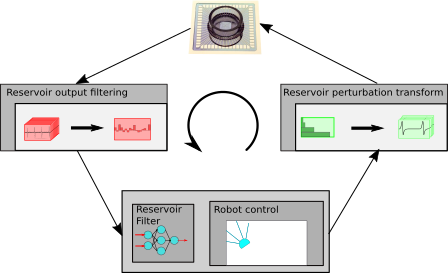
\includegraphics[width=0.5\textwidth]{fig/RCloop.png}
  \caption{Rough sketch.
    Some wavez
  }
  \label{figDataLoop}
\end{figure}
%
\section{Core Reservoir Computer}
%% As discussed in the previous chapter, the core reservoir computer is the
%% ideal reservoir readout layer and the perturbation generator while the remaining
%% functionality is abstracted away in the interface and feedback processor box.
%% The core reservoir computer consists of two parts, the robot control and the
%% reservoir readout layer.
The #core reservoir computer is comprised of a readout layer and a robot control
module.
\subsubsection{Readout Layer}
% skriv no fornuftig her da
The chosen readout layer is a simple feed forward neural network.
As mentioned in the background, the choice of using a network with multiple
layers as indicated in the figure means that a non-linear problem may be solved
entirely by the readout layer.
For the proof of concept the topology of the network is not fixed to a topology,
thus it is up to the experimenter whether a network with a single layer or one
with multiple layers should be used.
In fact, there is no strict requirement that the readout layer must be an
artificial neural network at all.
While it might seem a wise choice to use a readout layer that has similarities
with the reservoir itself, this line of thinking ignores the ``anonymization''
that happens between reservoir and reservoir computer, as shown in the fig
\ref{figGenericSpecific} in the previous chapter.
The final word on the choice of readout layer is that the artificial neural
network approach has the following benefits:
It can easily be extended from a linear to nonlinear classifier, and it is easy
to modify during an experiment.
\subsubsection{Robot Control}
The robot control is a simulator that controls an agent with 4 ``eyes'' in a box
world as shown in \ref{figGame}.
As with all other parts of the system, variables such as the amount of eyes, sight
range, the function between the output of the reservoir filter and robot
movement, max turn rate and max speed can be changed on a per-experiment basis,
but as long as they are ``good enough'' there is little scientific value in
exploring them and they should remain fixed.
The goal of the ``game'' is for the robot to not collide with walls.
Since the best way to avoid this is to simply run in circles, the performance is
evaluated by how close the agent came to crashing in a series of trials where
the agent is faced towards the wall at different angles as shown in fig [TODO].
Since the actions of the robot are decided by the output of the readout layer it
the action of the agent indirectly depends on the evaluation function since it
is this evaluation that shapes the next readout layer.
\begin{figure}[h!]
  \centering
  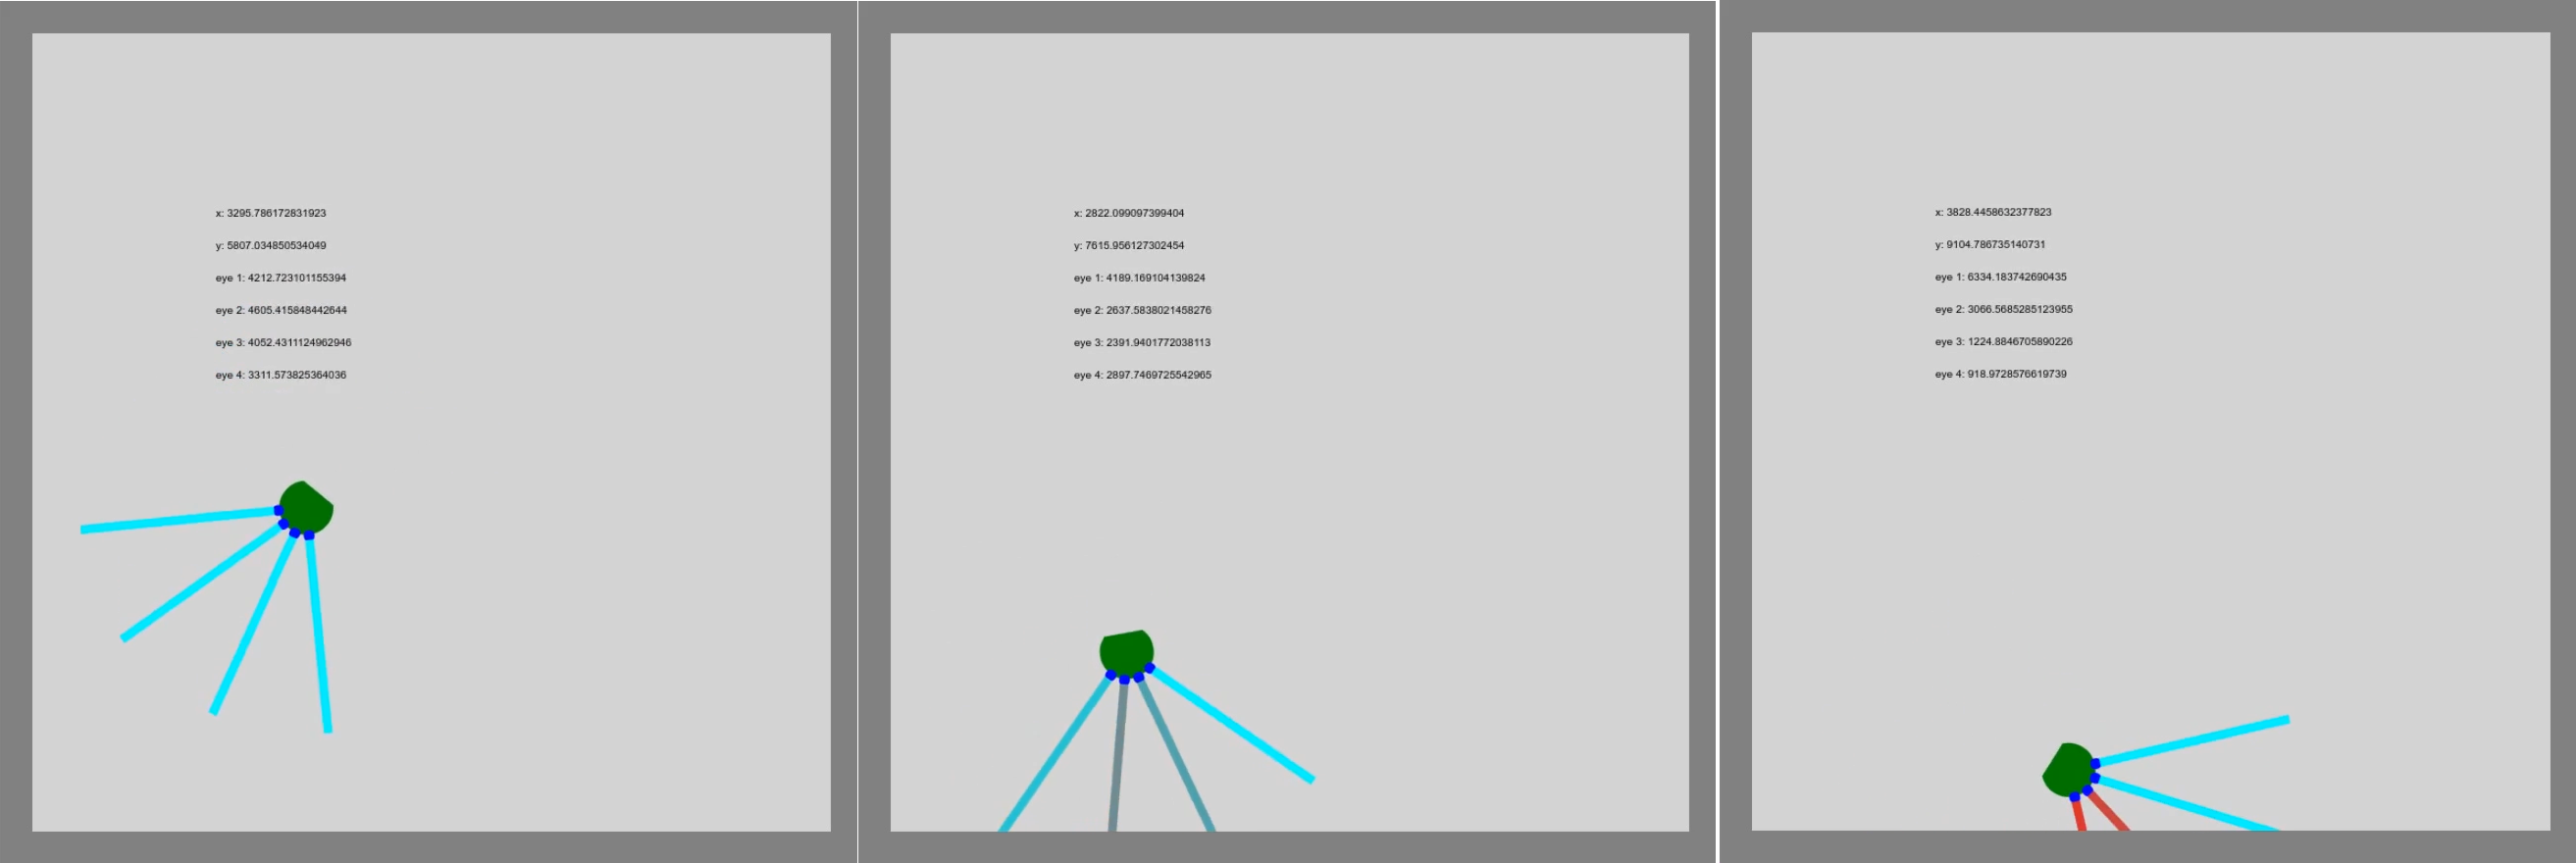
\includegraphics[width=1\textwidth]{fig/TAC/game2.png}
  \caption{The cyborg doing its thing}
  \label{figGame}
\end{figure}
% \begin{figure}[h!]
%   \centering
%   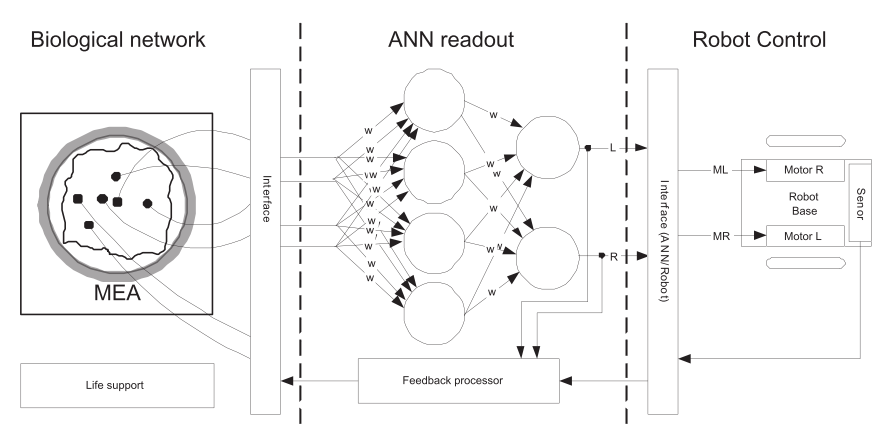
\includegraphics[width=1\textwidth]{fig/cyborg_overview.png}
%   \caption{A simple conceptual cyborg.}
%   \label{cyborgOverviewSimple}
% \end{figure}
\section{Reconfiguration Loop}
The reconfiguration loop, shown in \ref{figReconfLoop} is the dataflow
responsible for the on-line reconfiguration of the reservoir readout layer.
On experiment start the reservoir filter reconfigurator supplies the readout
layer module with a set of weights for the artificial neural network and records
the resulting behavior.
Each attempt is scored according to a scoring function as described in the
previous section, and from this the reservoir filter reconfigurator generates
new readout layers.
The chosen method of readout layer generation is a \emph{genetic algorith}
because of its ease of implementation and relative lack of bias.
\begin{figure}[h!]
  \centering
  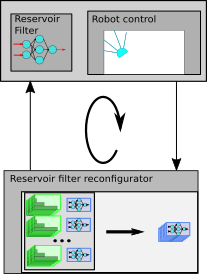
\includegraphics[width=0.5\textwidth]{fig/reconfigLoop.png}
  \caption{Rough sketch.
    Some wavez
  }
  \label{figReconfLoop}
\end{figure}
\section{Parameter Space}
% Noe fornuftig her I guess
\cleardoublepage

%%% Local Variables:
%%% mode: latex
%%% TeX-master: "../main"
%%% End:
